
\documentclass[book]{memoir}
\usepackage{color,graphicx}

\usepackage{wrapfig}
\definecolor{ared}{rgb}{.647,.129,.149}
\renewcommand\colorchapnum{\color{ared}}
\renewcommand\colorchaptitle{\color{ared}}
\chapterstyle{pedersen}
\setsecheadstyle{\color{ared}\Large\bfseries\memRTLraggedright}

%-----------------
%Fonts
%-----------------
%\usepackage{fourier}

\usepackage{fontspec}
\setmainfont{Linux Libertine}

%------------------------------

\usepackage[hidelinks]{hyperref}

\hypersetup{
  colorlinks,
  linkcolor=black,
  urlcolor=ared}
 
\usepackage{verbatim}
\usepackage[usenames,dvipsnames,svgnames,table]{xcolor}



\setlength{\parindent}{0pt}
\nonzeroparskip

% New Stuff--------------
\newcommand*{\plogo}{\fbox{$\mathcal{PL}$}} % Generic publisher logo
\usepackage{graphicx} % Required for box manipulation

\newcommand*{\rotrt}[1]{\rotatebox{90}{#1}} % Command to rotate right 90 degrees
\newcommand*{\rotlft}[1]{\rotatebox{-90}{#1}} % Command to rotate left 90 degrees

\newcommand*{\titleBC}{\begingroup % Create the command for including the title page in the document
\centering % Center all text

\def\CP{\textit{\Huge The Open Handbook}} % Title

\settowidth{\unitlength}{\CP} % Set the width of the curly brackets to the width of the title
{\color{LightGoldenrod}\resizebox*{\unitlength}{\baselineskip}{\rotrt{$\}$}}} \\[\baselineskip] % Print top curly bracket
\textcolor{Sienna}{\CP} \\[\baselineskip] % Print title
{\color{RosyBrown}\Large BOSTON UNIVERSITY} \\ % Tagline or further description
{\color{LightGoldenrod}\resizebox*{\unitlength}{\baselineskip}{\rotlft{$\}$}}} % Print bottom curly bracket

\vfill % Whitespace between the title and the author name

{\Large{Taylor and Vandenberg}}\\ % Author name

\vfill % Whitespace between the author name and the publisher logo

%\plogo\\[0.5\baselineskip] % Publisher logo
2013 % Year published

\endgroup}

\begin{document}

\titleBC % This command includes the title page
\thispagestyle{empty}
\newpage

\tableofcontents
\newpage

   %=============================================================
   %             +++++   PASTE CHAPTERS BELOW THIS LINE +++++
   %=============================================================

%-----------------------
% Academic Research
%-----------------------

\chapter{The Research Essay}
Research writing involves a number of critical skills: library research, critical thinking, the evaluation of sources, and the ability to synthesize information through summary, paraphrase, and quotation. Although synthesizing the thinking of others is an important part of the research essay, in its true form the research essay strives for much more than a mere re-presentation of what others have said on a particular topic or question. As \href{http://owl.english.purdue.edu/owl/resource/658/02/}{Jack Baker and Allen Brizee} state,

\begin{quote}A research paper is not simply an informed summary of a topic by means of primary and secondary sources. It is neither a book report nor an opinion piece nor an expository essay consisting solely of one's interpretation of a text nor an overview of a particular topic. Instead, it is a genre that requires one to spend time investigating and evaluating sources with the intent to offer interpretations of the texts, and not unconscious regurgitations of those sources. The goal of a research paper is not to inform the reader what others have to say about a topic, but to draw on what others have to say about a topic and engage the sources in order to thoughtfully offer a unique perspective on the issue at hand.\end{quote}

In high school you were perhaps asked to write a research paper on a predetermined topic. These essays were not true research essays in the sense that Baker and Brizee have in mind. Your projects were likely just retellings of what other scholars or writers have said on a topic. A true research essay, however, involves blazing a new path of inquiry where you produce original ideas, questions and arguments. In its true form, a research paper is a contribution to an ongoing conversation, a moment when you engage in dialogue with other important voices about a topic that you value.

\section{The Research Question}

Finding a research topic can often be an overwhelming experience. With so many things to choose from, finding a narrow focus can be difficult. However, before you can truly begin your library research you need to find a way to narrow your field of inquiry to a single research question or problem.

At the outset, your research questions will be rather general and mundane. But that is perfectly normal. We all have to start somewhere. Once you have a general topic of interest, however, you can move toward a more rigorous research phase.

As you begin your research, try to keep an open mind and allow yourself to be pulled in new directions. It is important to think of the research process as something more than a mere attempt to find information on a predetermined topic. Research is also a process of discovery where you encounter ideas and contemplate questions that you would have otherwise never imagined. For example, although a student might set out to write a paper on the Woodstock festival in the 1960s, she might end up writing a biography of \href{http://en.wikipedia.org/wikiMax_Yasgur}{Max Yasgur} (the owner of the farm where the festival took place) or an essay on how the rise in agribusiness resulted in a precipitous decline of family-run diary farming in upstate New York. A research project often contains many such unexpected twists and turns (and more often, dead ends).

\section{Finding A Topic}

If you are having difficulty finding a narrow topic of interest, one way to get started is to examine an organized list of \emph{every} subtopic that is related to your broader subject. Since the \href{http://catalog.loc.gov}{Library of Congress} assigns a series of \textbf{subject headings} to every published book, you can easily browse a meticulously categorized list of books that relate to your broader research subject. For example, if you want to write an essay on the nation of Iraq, you can perform a subject search with the search term "Iraq." The result will be an alphabetized list of \emph{every} subject that scholars have written on about Iraq\textemdash from agriculture to zoology. So, if you haven't yet found a narrow focus for your project, you can use the subject headings to "shop" for a subject that interests you. 

Subject searches are also a helpful means of finding additional sources once you have acquired one or more. For example, if you discover that historian Alan Taylor's book, \emph{The Civil War of 1812} is an important source for your project on border conflicts during the War of 1812, you can use the book's subject headings to find all of the other books that share that particular topic. The Library of Congress assigned Taylor's book the following three subject headings:

\begin{quote}
United States--History --War of 1812 --Social aspects

Ontario--History --War of 1812 --Social aspects

Northern boundary of the United States--History--19th century
\end{quote}

These subject headings are always included on the copyright page of a book, along with the name of the publisher and date of publication. However, the subject headings are also displayed in the library catalog entry for every book. In most libraries these subject headings are hyperlinked; clicking on any of them leads you to a list of every other book that shares that particular subject heading. Thus, if your research interest is United States -- History -- War of 1812 -- Social aspects, you can quickly find every other published book on that subject. 



Though Mugar's holdings are not nearly as large as the Library of Congress, you can perform subject searches by using the \href{http://library.bu.edu}{Subject Search} feature of our library catalog.

\section{Finding Background Information}

A research project should always begin with the reading of general background information about the topic. Before you can ask an intelligent question about your topic or contribute to an ongoing scholarly conversation, you need to develop a working knowledge of basic facts to serve as a foundation for your project. The best way to develop this basic understanding is to examine peer-reviewed reference works, such as encyclopedias.

Mugar library has a number of helpful reference resources in this regard. If you visit the \href{http://www.bu.edu/library/research/guides/research-guides}{\{Library Research Guides\}} link on the \href{http://www.bu.edu/library}{\{Mugar Homepage\}}, you will find an impressive array of organized reference materials like bibliographies, encyclopedias, and dictionaries. Most of them are fully digitized and do not even require a trip to the library. Always start your research project with reference works and gain a basic grounding of your topic before developing your research question or thesis.

Other helpful background information aids:

\begin{itemize}
\item \href{http://www.wikipedia.org}{\{Wikipedia\}}

\item \href{http://www.cia.gov/library/publications/the-world-factbook/}{\{CIA World Factbook\}}

\item \href{[http://www.oxfordreference.com.ezproxy.bu.edu}{\{Oxford Reference Online\}}

\end{itemize}
A word of warning about Wikipedia (and internet sources in general). It has not been through a process of peer review. The author of that article you're reading on \href{http://en.wikipedia.org/wiki/Weapon_of_mass_destruction}{\{WMD\}} could have been written or edited by a used car salesman. For that reason, it is unwise to use Wikipedia as a source for a research project. In addition, many professors will refuse to accept Wikipedia as a legitimate source. 

\section{Searching for Books}

Mugar library provides both \href{http://www.bu.edu/library}{\{simple\}} and \href{http://buprimo.hosted.exlibrisgroup.com:1701/primo_library/libweb/action/search.do?tab=default_tab&mode=Advanced&scp.scps=scope%3a%28BOSU%29%2cscope%3a%28BU_OAI%29%2cprimo_central_multiple_fe&vid=BU}{\{advanced\}} searching of the library catalog. The simple search feature provides you with an experience similar to Google. You can enter an author's name, the title of a book, or keywords. Once the search results are presented on the screen, use the "Refine my Results" links on the left of the page to limit the search to "print books" or "electronic books."

\section{Searching for Periodicals/Articles}

Periodicals are publications that are published at regular intervals, such as scholarly journals, magazines and newspapers. Examining periodicals\textemdash especially academic journals\textemdash is an important aspect of research. Since books often take a year or more to go through the process of peer review, editing, typesetting and printing before they become available for purchase, they often do not contain the most current information. Articles, on the other hand, appear in a far shorter period of time and generally contain the most up-to-date research. For that reason, you should perform a review of journal articles on your research topic to ensure that you are aware of recent discoveries, arguments, and debates within the academic community who share your research focus.

The librarians at Mugar library have created a convenient \href{http://www.bu.edu/dbin/ejournals/esources/alpha-es.php}{\{Periodical Index\}} that lists each of our periodical databases alphabetically. If you know the name of a particular journal or database, you can select it from the index and begin searching for information.

However, a common problem for undergraduate researchers is not knowing which databases or journals to search for information on a particular topic. Unless you are a professional scholar, it is difficult to know what the leading journals are in a particular field of study. Although an English professor would know that the academic journal \emph{PMLA} or the database JSTOR are excellent places to look for articles on Herman Melville's novel, \emph{Moby Dick}, the novice research wouldn't know where to begin. 

To help avoid this problem, our library has authored a broad collection of \href{http://www.bu.edu/library/research/guides/research-guides}{\{Research Guides\}} designed to help you locate the specific journals, periodical databases, and reference materials that are appropriate for each discipline or research topic. These are an indispensable resource for discovering peer-reviewed sources on your chosen topic. 

\section{Searching with Precision}

A common research problem is that your searches produce too many results. Rather than page through hundreds or thousands of search results, you should become familiar with powerful \textbf{Boolean searches} to make your search terms more precise. Boolean searches use what are known as \textbf{logical operators} to form search terms. The most common logical operators are AND, OR, and NOT. 

\subsection{AND}

Although it may seem counterintuitive, \textbf{AND} functions to \emph{limit or narrow} the number of sources you retrieve from a database. You can visualize the search of a large academic database or library catalog using the following diagram:
 
\begin{center}
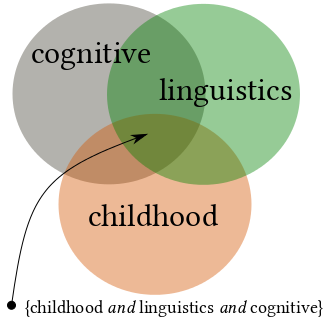
\includegraphics[width=.45\textwidth]{and3colors.png}
\end{center}

In the search depicted above, a student has requested articles that contain the subjects \textbf{cognitive}, \textbf{linguistics}, and \textbf{childhood}. Significantly, this particular search will only retrieve articles that contain \emph{all three terms}. In the diagram above, these results are referenced by the arrow. All the information represented by the other three circles will be excluded from the search results. Thus, even if an article contains two of the three search terms, it will be excluded from the results.

\subsection{OR}
Unlike the \textbf{AND} operator, \textbf{OR} seeks to \emph{broaden} a search, as in this example:

\begin{center}
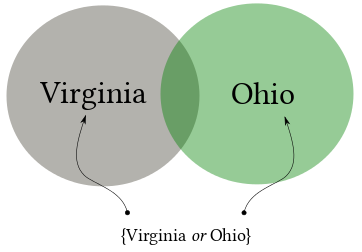
\includegraphics[width=.45\textwidth]{Orcolor.png}
\end{center}

In the search depicted above, a student has searched for the subjects Virginia \textbf{OR} Ohio. This search will return \emph{every} article having the subject of Virginia as well as \emph{every} article with the subject of Ohio. Unlike the \textbf{AND} search, where only articles containing \emph{both} terms are returned in the search results, the \textbf{OR} search yields every article on both subjects regardless of whether those subjects appear together in the same article. As a consequence, the \textbf{OR} search will produce far more results.

\subsection{NOT}
The Boolean operator \textbf{NOT} is used to \emph{subtract} or \emph{screen out} topics or keywords that are unwanted within the search results. 


\begin{center}
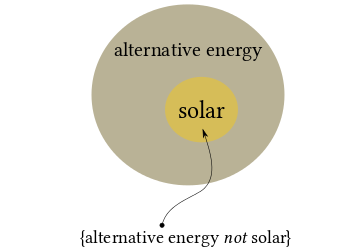
\includegraphics[width=.45\textwidth]{notcolor.png}
\end{center}


In the search depicted above, a student is researching alternative energy, but is not interested in solar energy. To remove all references to solar energy, the student has searched for \textbf{alternative energy}, but has removed any article from the search results that contain the subject \textbf{solar}. 

Alternatively, if you were researching the Norse explorers known as the Vikings, you might frequently find that your search results include unwanted information about the Minnesota Vikings football team. To resolve this problem, you can subtract these unwanted results by searching for: \textbf{Vikings not Minnesota} or \textbf{Vikings not football}.  

\subsection{Parenthetical Searches}

You can also use the various Boolean search terms in tandem using parenthetical constructions:

\begin{itemize}
\item (Ohio or Virginia) and unemployment
\item (cognitive and linguistics) not childhood
\end{itemize}
Using parentheses in a search results in the database query being performed according to the order of operations, like in math equations. In the first example, the search will combine all the articles that are on the subjects of \textbf{Ohio} or \textbf{Virginia}, creating a large collection of search results. Afterward, the search term \textbf{unemployment} will be applied to that collection, yielding the final search results. Similarly, the second example creates a large collection of results that share the subjects \textbf{cognitive} and \textbf{linguistics}, then all the items having the subject \textbf{childhood} are removed from the results.

\subsection{Exact Phrase}

Most Internet search engines and, increasingly, library catalogs default to the \textbf{AND} operator when multiple terms are entered. For example, if you search for \textbf{artificial intelligence}, the search algorithm will actually use the search phrase \textbf{artificial \emph{and} intelligence}. In some circumstances this will skew your search results.

To avoid this problem, you can instruct your search engine to perform an exact phrase search. This is performed by placing quotation marks around the exact words that you are searching for. In this example, you could search for "artificial intelligence". Now, your search results will only contain articles that use that exact phrase somewhere in the document.

\subsection{Truncation and Wild Cards}
\begin{itemize}
\item Manufact\** [truncation]
\item wom\**n [wild card]
\end{itemize}
If you search for the terms \textbf{steel and manufacturing}, your search results will not include results with the terms \textbf{manufacturer}, \textbf{manufacture}, \textbf{manufactured}, or \textbf{manufactures}. As a result, you may not discover articles or books that are important to your research. By truncating the word with an asterisk, you will gather all the relevant search results. 

Similarly, if you only search for \textbf{wom\emph{e}n}, you will miss out on the all the texts that mention \textbf{wom\emph{a}n}. By using the wild card asterisk, you will search both terms at the same time.

\section{Finding a Book in the Library}

Most research libraries use the Library of Congress (LC) classification system to organize their holdings. Each item in the library has a unique \textbf{call number} consisting of a series of numbers and letters that help you locate them on the library's shelves. When you look a book up in the library's catalog, you will find that it has been identified with a call number that looks like this: 

\begin{quote}
\hspace{.4in}{\huge F 24 .T39 1990}
\end{quote}

Let's break down the call number into its component parts:

\begin{quote}
\hspace{.4in}\begin{tabular}{ |l|l| }
  \hline
  F & Letter, or subject, line \\ \hline
  24 & Whole number line \\
  \hline
  .T39 & Cutter line \\ \hline
  1990 & Edition or date line\\ \hline
\end{tabular}
\end{quote}

\begin{itemize}
\item \textbf{The Letter line} describes the subject or discipline of the book. It also indicates \emph{the section (or floor)} where the book is shelved (consult your library's map and flooplan). The letter line will be between one and three letters long.
\item \textbf{The Whole Number Line} tells you which \emph{row} the book is on in the stacks. 
\item \textbf{The Cutter line} identifies the \emph{individual book}. The first letter of the Cutter line is usually the first letter of the author's last name.
\item \textbf{The Edition or Date line} tells you the year of publication to distinguish between editions.
\end{itemize}

To find this particular book, we would begin with the \textbf{Letter line}. Use the \href{http://www.bu.edu/library/mugar-memorial/about/floorplans/#f=floor-1}{floorplan map provided by the library} to determine the floor where all the \textbf{F }books are shelved. In this case, the book is located on the 4th floor of Mugar. Next, you will use the \textbf{Whole number line} to find the row of books where the 24s are held. As you walk through the stacks, look on the ends of each row of books for a sign describing the range of books held within the row. You might see a sign reading:

\begin{quote}
\hspace{.4in}{\huge F 7.4\textendash F 45.2}
\end{quote}

Since \textbf{F 24} is within this range, our book is within that row. Once in the proper row of shelves, proceed numerically until you find the 24s. Then, using the \textbf{Cutter line}, proceed alphabetically until you find the Ts. Then proceed numerically until you find .T39, the address of our book. 

As you can see, the call number should be read from left to right using alphabetical and numerical orders. Thus, a book with a Subject line \textbf{F }would be shelved \emph{before} a book with a Subject line \textbf{FA.} Similarly, a Cutter line that reads \textbf{.T39} is shelved \emph{after} \textbf{.T21}. 

\hspace{.4in}\textbf{Remember, with decimals .7 is bigger than .21!}

The LC numbers ensure that every book in a library will be organized in a uniform order. Thus, the book with call number \textbf{HE 8700.7 .P6T44 1983} in BU's Mugar library will have the identical call number in Boston College's O'Neil library. However, since every library is a unique building with different architecture and floorplans, you will need to consult a map before you try to locate your book.

Mugar Library has created \href{http://www.bu.edu/library/mugar-memorial/about/floorplans/#f=floor-1}{\{online maps and floorplans for their holdings\}} which you will need to locate books. 

\section{What if we don't have it?}
    
A common problem in academic research is discovering that a source that you require for a project is checked out, missing, or not owned by the library. There are a number of services available to you when you encounter such research problems.

\subsection{Boston Consortium Libraries}

A number of Boston-area colleges and universities have formed a library consortium designed to share resources and expand research options for the entire academic community. As students of Boston University, you may obtain borrowing privileges at any of the other 17 participating libraries. 

If you would like to see if a book is available at another \href{http://www.blc.org/members/current-members}{\{BLC\}} library, use a service called \href{http://www.bu.worldcat.org}{\{WorldCat Local\}}. With this service you can search every library in the BLC simultaneously to see if the book you require is available at another local institution. If the book is owned by another school and is not checked out at the time, you can request that the item be sent to our library free of charge. To request a book, click the green button labeled "Request Item." Once Mugar's circulation desk receives the item, they will inform you through email that the text is ready for pickup.

\subsection{Boston Library Consortium Card}
If you would like to check out a book at one of the other BLC member libraries in person, you may obtain borrowing privileges by applying for a \href{http://www.bu.edu/library/services/ill/blc-cards}{\{Boston Library Consortium Card\}}. To apply, fill out the online form and you will be contacted when your card is ready for pickup at Mugar's circulation desk.

\subsection{Interlibrary Loan}
If there is a book or article that you would like to read that is not available at any BLC library, you may request it from BU's Interlibrary Loan office. To request an item, visit the \href{http://illiad.bu.edu/illiad/bos/illiad.dll}{\{Interlibrary Loan\}} webpage, select the appropriate form (article, book, book chapter, etc.) and send your request electronically to the ILL office. The staff in the office will request your item from another library, who will ship the book to our library through the mail. 

\textbf{Please note}: Interlibrary Loan is the \emph{slowest} of all the available options for requesting research materials. Requests may take up to two weeks to be fulfilled. 


\section{Research Guides}

If you are performing research on a topic and do not know where to begin, Boston University Librarians have created an impressive collection of \href{http://www.bu.edu/library/guides/index-a-h.html}{\{Research Guides\}} that can help you find background information, periodical databases, and academic journals appropriate for your topic or discipline.

\section{Peer Review}

Peer review is a form of quality control in academic publishing. It ensures that the information that is published has been through a rigorous process of examination by other professionals in the field. Through the process of peer review, a variety of errors or mistakes can be eliminated before publication occurs. Thus, peer-reviewed sources should be preferred over any other kind of information. However, for a novice researchers, distinguishing between peer-reviewed and non-peer-reviewed sources can be challenging. So, how do you determine if a source is "scholarly" or peer-reviewed?

There are a number of things you can do to ensure that you are using peer-reviewed information. Many periodical databases, such as \href{http://www.jstor.org.ezproxy.bu.edu/jstor/}{\{JSTOR\}}, only contain peer-reviewed academic articles. Many other databases, such as \href{http://infotrac.galegroup.com.ezproxy.bu.edu/itweb/mlin_b_bumml?db=AONE}{\{Academic OneFile\}}, have a search limiters that you can select that will ensure that your search results only contain peer-reviewed sources. Other databases lack clear indications about the nature of their sources. If you are at any point confused about a source or database, ask your professor or one of the research librarians for assistance.

If those are not practicable, use these test criteria:
\begin{itemize}
\item Scholarly articles almost always publish the university affiliation of the professor/author. 

\item Scholarly articles \emph{always} have a Works Cited or bibliography page. 

\item Scholarly articles commonly have footnotes or endnotes. 

\item A good test is if you can find the journal at the dentist's office or on an airport magazine rack, then it isn't scholarly or peer-reviewed. \emph{Time}, \emph{Newsweek}, even the \emph{New York Times} are not considered peer-reviewed sources.
\end{itemize}

\section{The Oxford English Dictionary}

The \href{http://www.oed.com.ezproxy.bu.edu}{\{OED\}} is, without question, the greatest and most complete dictionary ever created. Many generations of scholars have made it their life's work. The OED systematically traces the etymology of words in the English language. \href{http://en.wikipedia.org/wiki/Etymology}{\{Etymology\}} is "the study of the history of words, their origins, and how their form and meaning have changed over time." Thus, with the OED, you can see when a word entered or exited the English language and how its meaning evolved over time. 

The OED is quite helpful when you are reading a novel, poem, or document that was written in a time period distant from our own. Since words fall out of use and the meanings of words change over time, it can often be difficult to interpret the meaning of the text in question. The OED exists to help us with this problem: you can think of it as a dictionary with a built-in time machine. 

To illustrate the utility of the OED, let's consider an example. In Anthony Trollope's 1864 novel entitled \href{http://www.gutenberg.org/files/4599/4599-h/4599-h.htm#c2}{\emph{The Small House at Arlington}}, the following bit of dialogue may be found:

\begin{quote} "I am not in Mr. Crosbie's confidence. He is in the General Committee Office, I know; and, I believe, has pretty nearly the management of the whole of it. I have heard Bernard say that he has six or seven young men under him, and that\textendash; but, of course, I don't know what he does at his office."

"I'll tell you what he is Bell; Mr. Crosbie is a swell." And Lilian Dale was right; Mr. Crosbie was a swell. [\dots]

 "I don't like those slang words, Lily."

"What slang words?"

"You know what you called Bernard's friend."

"Oh; a swell. I fancy I do like slang. I think it's awfully jolly to talk about things being jolly. Only that I was afraid of your nerves I should have called him stunning. It's so slow, you know, to use nothing but words out of a dictionary."
\end{quote}

What is "a swell"? The context here doesn't give away much. And Lily Dale's use of the word "swell" doesn't accord with our modern understanding of the word. In order to discover what this word meant to the 19th century audience who first read the novel, we need to consult the OED.

If we search the word "swell" in the \href{http://www.oed.com.ezproxy.bu.edu}{\{Quick Search\}} box of the OED, we can browse through the definitions which include "morbid swelling," "the condition of being swollen, distended or increased in bulk," "the rising or heaving of the sea," "a piece of land rising gradually and evenly," "a sound, esp. musical," "a contrivance for gradually varying the force of the tone in an organ," and a "lever in a loom."

None of the definitions seem particularly helpful. However, definition \textbf{9a} reads:

\begin{quote}\textbf{9a} \emph{colloq}. , orig. \emph{slang}. A fashionably or stylishly dressed person; hence, a person of good social position, a highly distinguished person. \end{quote}

This seems to be the sense in which Lilly Dale means to use the term. Furthermore, the OED explains that this particular sense for the word "swell" was in active use between 1786 and 1892. Since Trollope's novel was published between those dates, we can feel confident that this is the proper meaning of the word.
\section{Other Helpful Suggestions}

\subsection{Not all sources are equal}

How do you know if you can trust your source? Here are some suggestions for critically examining your sources:

\begin{itemize}
\item \textbf{Examine the credentials of the author}. What is their educational background? Do they have an advanced degree in the subject that they are writing about? Are they affiliated with any major institutions\textemdash such as a university or government department? Does the author have a respected publication record that is frequently cited by other experts in the field?

\item \textbf{Examine the date of publication}. When was the book or article you are reading published? Since new discoveries and ideas are produced every day, it is important to consult the most recent sources on your research subject. Generally, the most current source should be preferred over something that is decades old.

\item \textbf{Determine if the source has been peer-reviewed}. Peer review is a form of quality control in academic publishing. It ensures that the information that is published has been through a rigorous process of examination by professionals in the field. A peer-reviewed source should be preferred over any other kind of information.

\item \textbf{Be wary of Internet sources}. If your source comes from the Internet, you should take extra precaution to verify the source's trustworthiness. Most sites on the Internet are not peer-reviewed sources of information. Misleading, politically motivated, and even propagandistic content often masquerades as objective information on blogs, websites, and discussion boards. 
\end{itemize}

\subsection{Taking notes}

Now that you have some research materials in front of you, either at the library or at home, it's time to make them useful to you. Taking notes on a source is a crucial skill. If you'd rather take notes on your computer, try the free open-source program called \href{http://rasm.ods.org/keepnote}{\{Keepnote\}}.

\subsection{Raid the Bibliography}

Occasionally, students find one or two sources on a topic and then despair of finding any more. However, with just one excellent article or book, you can easily generate additional research leads. When you find a book or article that relates to your project, scour the bibliography to see what books and articles the author used to produce his or her work. Make lists of the most promising sources by writing down all the bibliographic information in a research journal. Locate these sources in the library and then repeat the process. By using this technique of routinely following up on sources cited in bibliographies, you can generate a surprisingly large number of books and articles on your topic in a relatively short time.

\subsection{Keep a Research Journal}

Keeping a research journal is an important habit to develop. Every student or professor has had the unsettling realization that they have used a quotation in their writing but have no recollection of where the quote came from. Many hours can be consumed retracing steps. Frequently, source materials are never located again. To avoid this problem, keep a research journal where you record the bibliographic information of each source you read or browse. This way you can quickly locate the information again. 

Although a paper notebook works well as a research journal, there are some very promising electronic alternatives. This bibliographic software can maintain a record of your sources, help you take notes, and even automatically produce perfectly formatted bibliography pages for your essays. For Mac users, there is \href{http://www.sonnysoftware.com/}{\{Bookends\}}. PC users should consider \href{http://www.biblioscape.com}{\{Biblioscape\}}. However, the free and open-source option known as \href{http://zotero.org}{\{Zotero\}} is perhaps the best option of all.


\end{document}